\section{Results}
\label{sec:results}

In this section, we numerically evaluate the quantum resources required for block-encoding various operators using LOBE.
The spacetime costs that we analyze include: the number of T gates, the number of non-Clifford single qubit rotations, the number of block-encoding ancillae, the maximum number of qubits required, and the rescaling factor imposed on the resulting block-encoding.

We compare the LOBE constructions presented in Section \ref{sec:ladder-op-oracles} to techniques that first expand the ladder operators in the Pauli basis and then block-encode the resulting linear combinations of Pauli operators using LCU.
The Jordan-Wigner transformation \cite{jordan-wigner} is used to expand fermionic ladder operators in the basis of Pauli operators, while, the Standard Binary encoding \cite{standard-binary} is used to expand bosonic ladder operators.

The first Pauli-based method we compare against will be referred to as ``Pauli Expansion''.
In this method, the respective Pauli transformations are applied to the ladder operators and fully expanded, resulting in a single linear combination of Pauli operators.
This linear combination, which describes the full operator, is then block-encoded using the LCU framework.

The second Pauli-based method we compare against will be referred to as ``Piecewise Pauli''.
In this method, each product of ladder operators acting on a single mode is expanded in the Pauli basis and then block-encoded using the LCU framework.
These block-encodings of the ladder operators acting on each mode are then combined together to produce a block-encoding of the full operator using the techniques described in subsections \ref{subsec:lco} and \ref{subsec:be-products}.

In the following subsections, we benchmark these three different block-encoding methods for various types of operators.
First, we analyze the associated spacetime costs for block-encoding several classes of operators which appear in many second-quantized operators.
Then, we present the spacetime costs for block-encoding Hamiltonians associated with various models that arise in quantum field theory.
These models include Hamiltonians derived from two non-relativistic models - the quartic harmonic oscillator and the static massive Yukawa - and two fully relativistic models - $\phi^4$ theory and the full massive Yukawa.

For all block-encodings, we will assume that all terms are normal ordered and that the identity term is removed.
Normal ordering each term ensures that the accuracy of the output state is not affected by the bosonic cutoff.
The identity term is removed since it artificially inflates the rescaling factor and only results in a constant shift in the spectrum of the Hamiltonian, however, if required it can be included with a negligible increase in spacetime quantum resources.

The results presented in this section are generated using a software library called LOBE which has been made open-source \cite{}.
The circuits are implemented using Cirq \cite{cirq} and block-encodings are numerically verified for circuits of up to 18 qubits.
OpenParticle \cite{openparticle}, a software library for the construction and manipulation of fermionic, antifermionic, and bosonic ladder operators, is used to define the operators.
The Symmer software library \cite{} is also used for various subroutines, including, but not limited to, expanding the ladder operators in the Pauli basis.
The software library \cite{grover-rudolph-github} is used to determine the rotation angles required for arbitrary state-preparation using Grover-Rudolph.


\subsection{Components}

In this subsection, we numerically benchmark the spacetime cost of LOBE constructions for three different sets of operators.
We compare the cost of the constructions with the two methods outlined above which require expanding the ladder operators in the Pauli basis.

\begin{figure*}
    \centering
    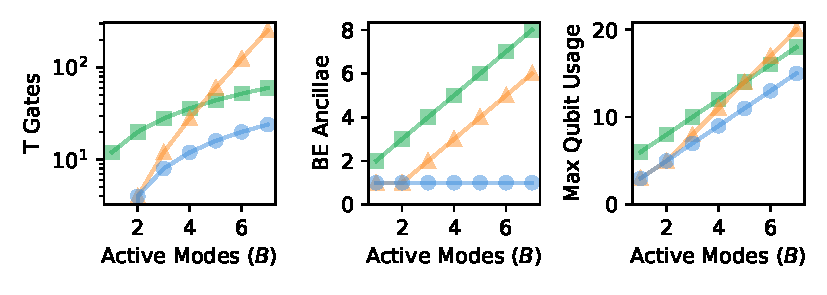
\includegraphics[width=12cm]{figures/fermionic-hc-comparison.pdf}
    \caption{
        \textbf{Spacetime Cost to Block-Encode $O = b_0 b_1 \hdots b_{B-1} + h.c.$}
        The number of T gates (left), block-encoding ancillae (middle), and maximum number of qubits used (right) are shown as a function of the number of active modes ($B$).
        Results for ``Pauli Expansion'' are shown as the orange triangles, results for ``Piecewise Pauli'' are shown as the green squares, and results for LOBE are shown as the blue circles.
        For this operator, all block-encodings use zero non-Clifford rotations.
        Both ``Pauli Expansion'' and LOBE have optimal rescaling factors ($\lambda = 1$) while ``Piecewise Pauli'' has a rescaling factor of $\lambda = 2$.
    }
    \label{fig:fermionic-hc-comparison}
\end{figure*}

The first set of operators we examine are described by a product of fermionic annihilation operators acting on different modes plus its hermitian conjugate: $b_0 b_1 \hdots b_{B-1} + h.c.$.
The numerical spacetime costs of the three block-encoding methods for these operators are shown as a function of the number of active modes ($B$) in Figure \ref{fig:fermionic-hc-comparison}.
Notably, the spacetime costs for LOBE and ``Pauli Expansion'' are identical for $B = 1$ and $B = 2$.
However, the number of required T gates scales exponentially with $B$ for ``Pauli Expansion'', yet scales linearly for LOBE.
Additionally, the LOBE constructions only require a single block-encoding ancilla, independent of $B$,while both Pauli-based methods require a number of block-encoding ancillae that scale linearly with $B$.

\begin{figure*}
    \centering
    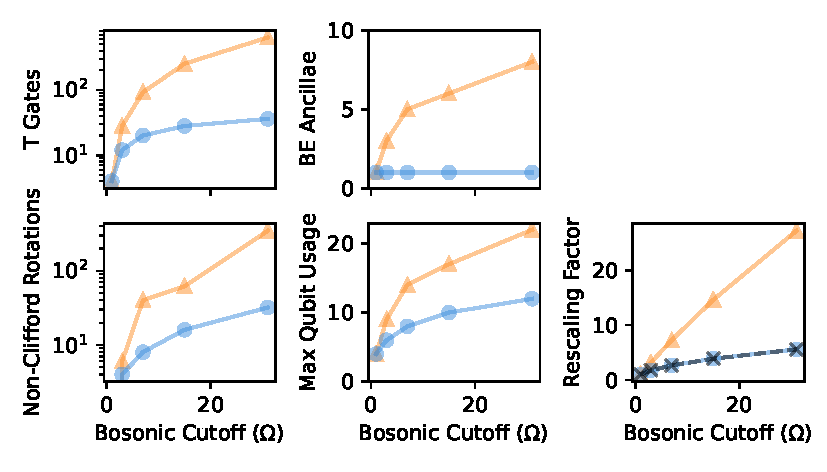
\includegraphics[width=14cm]{figures/bosonic-comparison.pdf}
    \caption{
        \textbf{Spacetime Cost to Block-Encode Bosonic Annihilation Operator}
        The number of T gates (upper-left), number of non-Clifford rotations (lower-left), block-encoding ancillae (upper-middle), maximum number of qubits used (lower-middle), and rescaling factor (lower-right) are shown as a function of the bosonic occupation cutoff ($\Omega$).
        Results for the Pauli (LCU) method are shown as the orange triangles and results for LOBE are shown as the blue circles.
        The optimal rescaling factor, which is given by the L2 norm of the matrix representing the bosonic annihilation operator with fixed $\Omega$, is shown as the dashed black crosses. 
    }
    \label{fig:bosonic-comparison}
\end{figure*}

The second set of block-encodings we consider is those that encode a single bosonic annihilation operator ($a$) with an increasing bosonic occupation cutoff ($\Omega$).
Since there is only a single operator, both Pauli methods result in the same construction therefore we refer to these constructions by ``Pauli (LCU)''.
The numerical spacetime costs and rescaling factors of the Pauli (LCU) and LOBE block-encodings are shown in Figure \ref{fig:bosonic-comparison}.
The LOBE constructions result in block-encodings with fewer required resources for all metrics as compared to the Pauli (LCU) method.
Notably, the number of required T gates scales logarithmically with $\Omega$ for LOBE, yet scales roughly linearly for the Pauli (LCU) method.
Additionally, the number of block-encoding ancillae is constant ($1$) regardless of $\Omega$ for LOBE, yet scales logarithmically for the Pauli (LCU) method.
Lastly, the LOBE construction results in a rescaling factor that matches the operator norm (optimal), while the Pauli (LCU) construction results in a larger rescaling factor.

\begin{figure*}
    \centering
    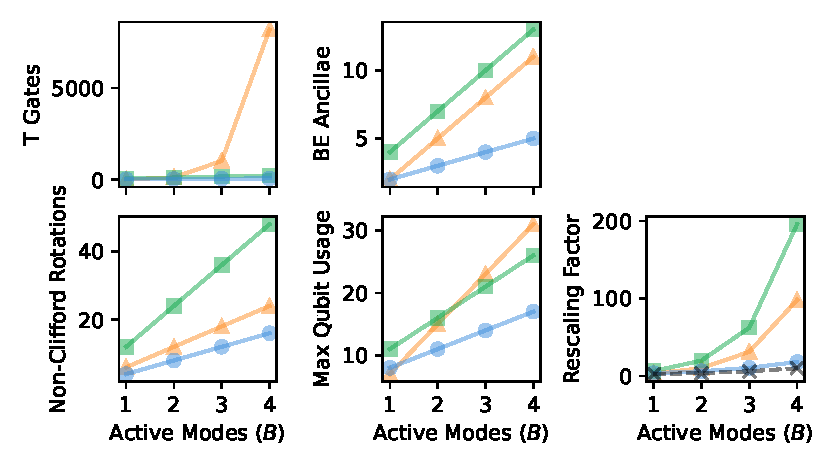
\includegraphics[width=14cm]{figures/bosonic-hc-comparison.pdf}
    \caption{
        \textbf{Spacetime Cost to Block-Encode $O = a_0 a_1 \hdots a_{B-1} + h.c.$}
        The number of T gates (upper-left), number of non-Clifford rotations (lower-left), block-encoding ancillae (upper-middle), maximum number of qubits used (lower-middle), and rescaling factor (lower-right) are shown as a function of the number of active modes ($B$).
        The bosonic cutoff is fixed to $\Omega = 3$ for all data points.
        Results for ``Pauli Expansion'' are shown as the orange triangles, results for ``Piecewise Pauli'' are shown as the green squares, and results for LOBE are shown as the blue circles.
        The optimal rescaling factor, which is given by the L2 norm of the matrix representing the operator with $\Omega = 3$, is shown as the dashed black crosses.
    }
    \label{fig:bosonic-hc-comparison}
\end{figure*}

The third set of operators we analyze are given as a linear combination of a product of bosonic annihilation operators acting on different modes plus its hermitian conjugate: $a_0 a_1 \hdots a_{B-1} + h.c.$.
The numerical spacetime costs of the various block-encoding constructions for these operators with $\Omega = 3$ are shown in Figure \ref{fig:bosonic-hc-comparison}.
Notably, the overall time-complexity scales linearly with $B$ for the LOBE and ``Piecewise Pauli'' constructions, while it scales exponentially for ``Pauli Expansion''.
For the space complexity metrics, all methods scale linearly with $B$, yet the LOBE constructions have both the smallest prefactor and numerical values.
Finally, the LOBE construction results in the lowest rescaling factor of all constructions.

In certain cases - such as when the number of active modes is small or the bosonic occupation cutoff is low - the ``Pauli Expansion'' construction can lead to lowest spacetime costs.
However, when the number of active modes is large or the bosonic occupation cutoff is high, the LOBE constructions lead to the lowest spacetime costs.
For all components analyzed here, the ``Piecewise Pauli'' constructions have similar asymptotic scalings compared to LOBE, but result in larger numerical spacetime costs.
For this reason, the ``Piecewise Pauli'' construction will be omitted when benchmarking full systems.

\subsection{Quartic Harmonic Oscillator Results}
\label{sec:qosc_results}

The quartic harmonic oscillator \cite{PhysRev.184.1231, girguś2024spiralflowquantumquartic, wójcik2012applicationnumericalrenormalizationgroup} is an extension of the standard harmonic oscillator with an additional non-linearity of the form $g \varphi^4$, where $g$ is an arbitrary constant that dictates the strength of the interaction, and $\phi$ is a bosonic field.
This leads to the Hamiltonian $H = \frac12\dot\phi^2 + \frac{m}{2}\phi^2 + gm^3\phi^4 $, where $\phi$ is composed of a single mode.
$m$ is the mass of the bosonic particle, and $\dot \phi$ represents the time derivate of the field.

In a second-quantized, dimensionless form, the Hamiltonian can be written as:
\begin{equation}
    \label{eq:qosc}
    H = a^\dagger a + g\left(a + a^\dagger \right)^4
\end{equation}
where there is only one bosonic mode.

After expanding the product, normal ordering all terms, and removing the constant offset, this Hamiltonian can be written as a linear combination of $8$ terms consisting of three pairs of operators plus their hermitian conjugates and two operators that are their own hermitian conjugates:
\begin{equation}
    \begin{split}
        H = &(12g + 1) a^\dagger a + 6g a^{\dagger^2} a^2 + 6g \left(a^{\dagger^2} + a^2 \right) \\
        + &4g \left(a^{\dagger^3} a + a^\dagger a^3 \right) + g \left(a^{\dagger^4} + a^4 \right)
    \end{split}
\end{equation}

\begin{figure*}
    \label{fig:qosc}
    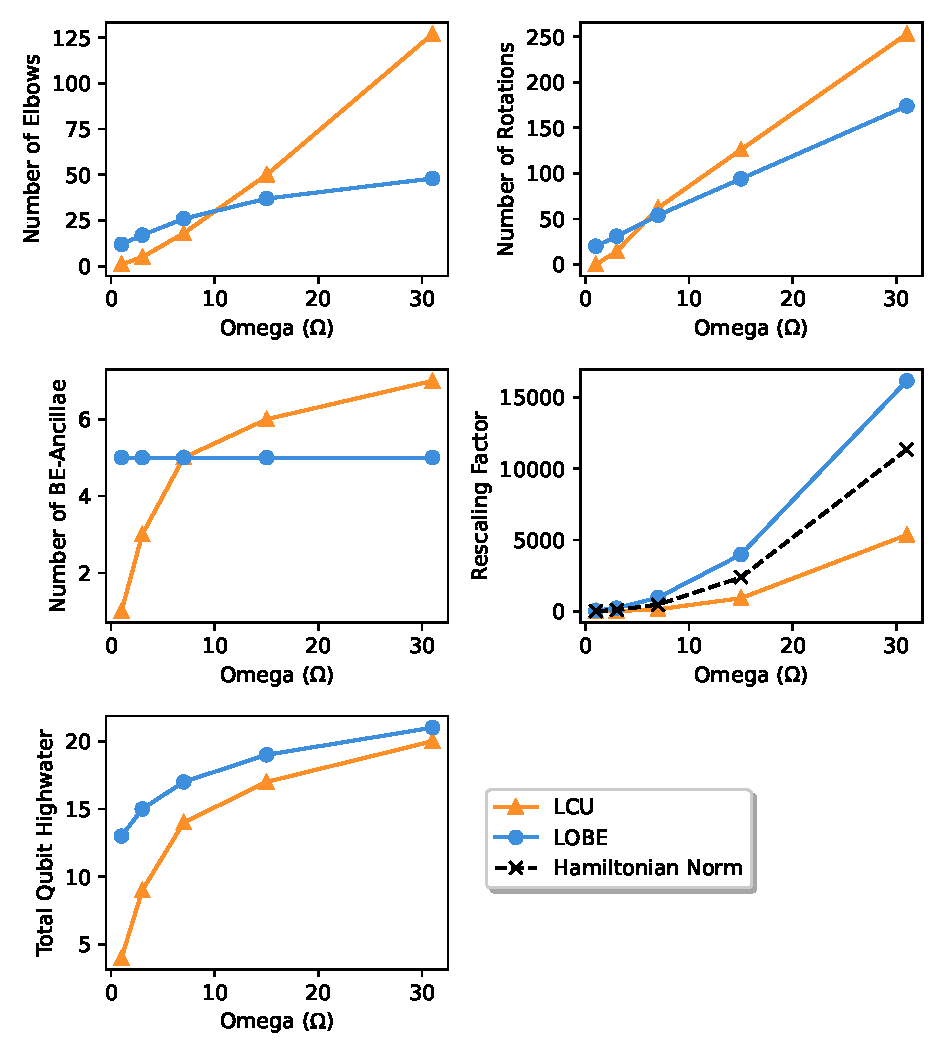
\includegraphics[width = 16cm]{figures/quartic_oscillator.pdf}
    \caption{
        \textbf{Quartic Harmonic Oscillator}
        The number of T gates (upper-left), number of non-Clifford rotations (lower-left), block-encoding ancillae (upper-middle), maximum number of qubits used (lower-middle), and rescaling factor (lower-right) are shown as a function of the bosonic occupation cutoff ($\Omega$).
        The parameter $g$ is set to $1$ for all data points.
        Results for the Pauli Expansion method are shown as the orange triangles and results for LOBE are shown as the blue circles.
        The optimal rescaling factor, which is given by the L2 norm of the Hamiltonian, is shown as the dashed black crosses.
    }
\end{figure*}

In Figure \ref{fig:qosc}, we show the scaling of the spacetime costs associated with both the LOBE and Pauli Expansion block-encodings as a function of the bosonic occupation cutoff ($\Omega$).
For small values of $\Omega$, the Pauli Expansion block-encodings result in lower spacetime costs, however, the LOBE constructions have favorable scaling and therefore a crossover point is seen.

For the time-complexity, this crossover occurs at $\Omega = 15$ for the number of T gates and $\Omega = 7$ for the number of non-Clifford rotations.
For the space-complexity, this crossover occurs at $\Omega = 7$ for the number of block-encoding ancillae and $\Omega = 31$ for the maximum number of qubits.
Finally, for the rescaling factor, this crossover occurs at $\Omega = 31$.

\subsection{Massive Static Yukawa}
\label{sec:static_yukawa}

The next simplest model that we consider is a non-relativistic approximation to the Yukawa model, which is commonly referred to as the massive static Yukawa model \cite{PhysRevD.103.014021}.
This model is taken as the limit of the full Yukawa model of infinitely heavy fermions, and bosons at rest relative to the fermions that emit/absorb them.

The second-quantized Hamiltonian for this model is given by:
\begin{equation}
    \label{eq:static-yukawa}
    H = C_f b^\dagger b + C_b a^\dagger a + g b^\dagger b \left( a + a^\dagger \right)
\end{equation}
where $C_f$ ..., $C_b$ ..., and $g$ ... \ws{@Gus}.
In this model, there is one fermionic mode and one bosonic mode so the indices on each mode are omitted. 

\begin{figure*}
    \label{fig:static_yukawa}
    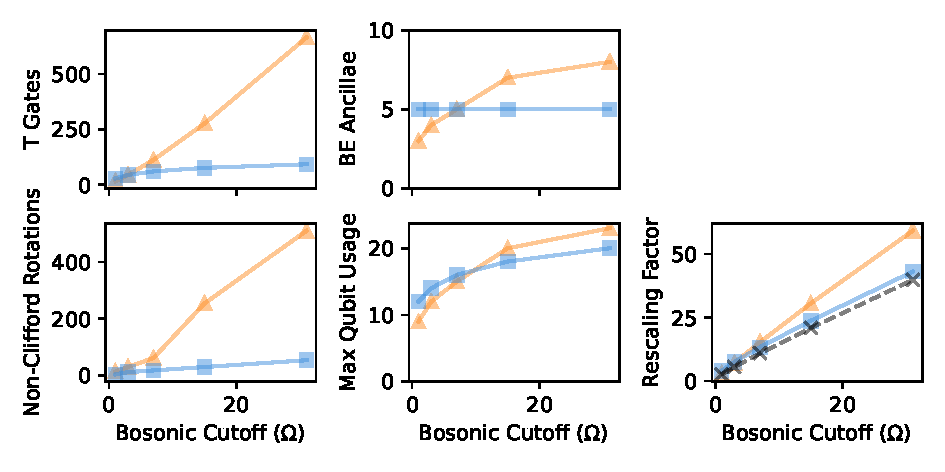
\includegraphics[width = 16cm]{figures/static_yukawa.pdf}
    \caption{
        \textbf{Static Massive Yukawa}
        The number of T gates (upper-left), number of non-Clifford rotations (lower-left), block-encoding ancillae (upper-middle), maximum number of qubits used (lower-middle), and rescaling factor (lower-right) are shown as a function of the bosonic occupation cutoff ($\Omega$).
        The parameters $C_f$, $C_b$, and $g$ are set to $1$ for all data points.
        Results for the Pauli Expansion method are shown as the orange triangles and results for LOBE are shown as the blue circles.
        The L2 norm of the Hamiltonian is shown as the dashed black crosses.
    }
\end{figure*}

As this model is restricted to one fermionic and one bosonic mode, we compare the spacetime costs of the different block-encoding methods as a function of the bosonic occupation cutoff ($\Omega$).
Similar to the quartic harmonic oscillator, the Pauli Expansion method results in lower spacetime costs when the bosonic cutoff is low.
However, the LOBE constructions have better asymptotic scaling with resect to $\Omega$ and crossover points exist for all metrics, above which LOBE results in lower cost constructions.

For the time-complexity, this crossover point occurs at $\Omega = 3$ for the number of T gates and the LOBE constructions require fewer non-Clifford rotations at all values of $\Omega$.
For the space-complexity, this crossover point occurs at $\Omega = 7$ for the number of block-encoding ancillae and $\Omega = 15$ for the maximum number of qubits.
Finally, for the rescaling factor, this crossover point occurs at $\Omega = 15$.
\subsection{$\phi^4$ Results}
\label{sec:phi4_results}

Any field theory is defined at the level of a Lagrangian.
For $\phi^4$ theory is given as
\begin{equation}
    \mathcal{L} = \frac12 \left(\partial_\mu \phi \right)^2 - \frac{m^2}{2}\phi^2 - g\phi^4.
\end{equation}

To obtain a Hamiltonian from a Lagrangian, a Legendre transformation is performed, in which an explicit set of coordinates must be chosen. 
The set of coordinates used in this paper, which lead to the simplest forms of the corresponding Hamiltonians, are front form (lightfront) coordinates \cite{Dirac1949}.
A discussion on lightfront coordinates will be given in appendix \ref{subsec:qft-hamiltonians}.

The $\phi^4$ Hamiltonian can be written as:
\begin{align}
    H = \sum_i &c_i a_i^\dagger a_i + \sum_{ijkl}c_{ijkl} \left(a_i^\dagger a_j^\dagger a_k^\dagger a_l + h.c. \right) + \nonumber\\
    &\sum_{ijkl}c_{ijkl}a_i^\dagger a_j^\dagger a_k a_l
\end{align}
where the values of the coefficients are omitted for brevity, but can be determined numerically.

Unlike the Quartic Harmonic Oscillator and the Static Massive Yukawa model, $\phi^4$ theory is defined based on a discretization of momentum modes.
In lightfront field theories, it is common to refer to the resolution of the model, which dictates the size of the momentum grid or the total number of momentum modes.
For those unfamiliar, the resolution can be thought of analogously to the molecular orbital basis in quantum chemistry simulations.
A further discussion on the physical meaning of resolution will be given in appendix \ref{subsec:qft-hamiltonians}.

\begin{figure*}
    \label{fig:phi4}
    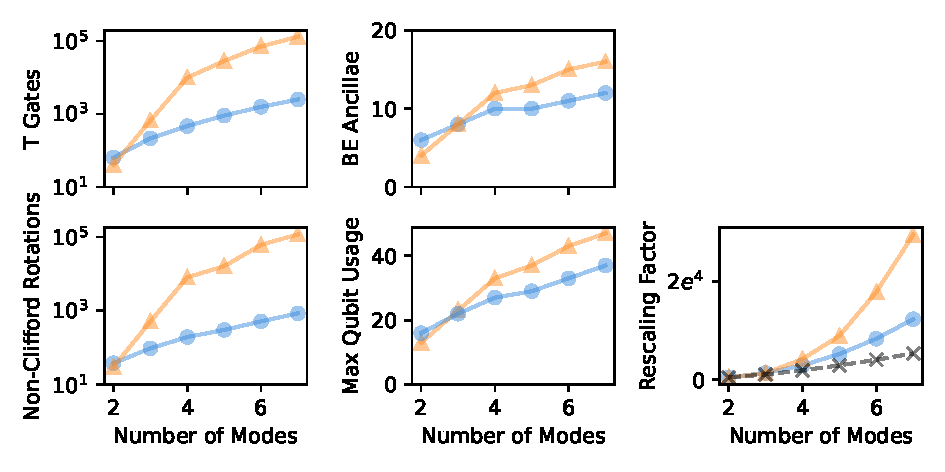
\includegraphics[width = 16cm]{figures/phi4-resolution-3.pdf}
    \caption{
        \textbf{$\phi^4$}
        The number of T gates (upper-left), number of non-Clifford rotations (lower-left), block-encoding ancillae (upper-middle), maximum number of qubits used (lower-middle), and rescaling factor (lower-right) are shown as a function of the number of momentum modes.
        The bosonic cutoff is fixed to $\Omega = 3$ and the parameters $g$ and $m_b$ are set to $1$ for all data points.
        Results for the ``Pauli - Expansion" method are shown as the orange triangles and results for LOBE are shown as the blue circles.
        The optimal rescaling factor, which is given by the L2 norm of the Hamiltonian, is shown as the dashed black crosses.
    }
\end{figure*}

Since the previous results establish that LOBE constructions are generally preferred when the bosonic cutoff is large, here we chose to look at the spacetime cost as a function of the total number of momentum modes.
In Figure \ref{fig:phi4}, we show the scaling of the spacetime costs associated with both the LOBE and Pauli Expansion block-encodings as a function of the number of modes.
For these estimates, the bosonic cutoff is fixed to $\Omega = 3$.
When the number of modes is small (low resolution), the LOBE and Pauli Expansion constructions require similar spacetime costs, with the Pauli Expansion block-encodings requiring \ws{one} fewer block-encoding ancilla when there are only two modes.
For higher resolutions (more modes), the LOBE constructions require signficantly fewer T gates and non-Clifford rotations, in addition to requiring fewer block-encoding ancillae, using fewer total qubits, and having smaller rescaling factors.
Notably, when $7$ momentum modes are used, the time cost for the LOBE construction is approximately two orders of magnitude smaller than the Pauli Expansion construction.

\subsection{Full Yukawa Results}
\label{sec:yukawa_results}

The first interacting field theory between different types of particles studied is generally the Yukawa model.
This is a theory of interacting fermions and bosons which can be used as a model of the strong nuclear force between hadrons.
The Lagrangian for this model is given as

\begin{equation}
    \label{eq:yukawa-lagrangian}
    \mathcal{L} = \bar \psi \left(i\gamma^\mu \partial_\mu - m \right)\psi + \frac{1}{2}\partial_\mu \phi \partial^\mu \phi - \frac{1}{2}\mu^2\phi^2 - g\bar \psi \psi \phi,
\end{equation}

The Hamiltonian can be written, again with coefficients obscured, as:

\begin{align}
    \begin{split}
        H = &\sum_i c_i b_i^\dagger b_i + \sum_i c_i d_i^\dagger d_i + \sum_i c_i a_i^\dagger a_i + \\
        &\sum_{ijk}c_{ijk}\left(b_i^\dagger b_j a_k^\dagger + h.c. \right) + \sum_{ijk}c_{ijk}\left(d_i^\dagger d_j a_k^\dagger + h.c. \right) + \\
        &\sum_{ijk}c_{ijk}\left(b_i^\dagger d_j^\dagger a_k + h.c. \right) + \sum_{ijkl}c_{ijkl}b_i^\dagger b_j a_k^\dagger a_l + \\
        &\sum_{ijkl}c_{ijkl}d_i^\dagger d_j a_k^\dagger a_l + \sum_{ijkl}c_{ijkl}\left(b_i^\dagger d_j^\dagger a_k a_l + h.c. \right)
    \end{split}
\end{align}

Unlike $\phi^4$ theory, the Yukawa model involves another type of field, a fermionic (Dirac) field $\psi$ describing fermionic particles.
$\bar \psi$ is the conjugate Dirac field, $m_f$ is the mass of the fermion, $m_b$ is the mass of the boson, and $g$ again describes the strength of the interaction.
